\documentclass[12pt]{article}

\usepackage{pdflscape}
\usepackage[margin=0.8in]{geometry}
\usepackage{titling}
\usepackage{graphicx} %Required for diagrams
\usepackage[hidelinks]{hyperref}
\usepackage{color}
\usepackage{framed}
\usepackage{epsfig}
\usepackage{epstopdf}

\begin{document}

\begin{titlepage}
	\begin{center}
		
		\begin{figure}[t]
			\centering
			
\includegraphics[width=350px]{images/UP_Logo.png}
		\end{figure}
		
		% Title
		\textsc{\large Project Tender} \\ 
		\vspace{2cm}
		\textbf{\Huge Project: RMB's Data Lake} \\ 
		\textsc{\large Client: RMB} \\ 
		\vspace{2cm}
		\textbf{\Huge Team: Team Name } \\ 
		
		%\begin{minipage}{0.4\textwidth}s
		\begin{flushright} \large
			Armand Pieterse \emph{u12167844} \newline
			Kgomotso Sito 		\emph{u12243273} \newline
			student name		\emph{uXXXXXXXX} \newline
			Sphelele Malo 	\emph{u12247040} \newline
			\end{flushright}
		%\end{minipage}
		\textsc{\small Department of Computer Science, University of Pretoria}
		
		\vfill
		
	Here's a link to \href{https://github.com/SpheMalo/COS-301-Main-Project.git}{GitHub}.\\
	\url{https://github.com/SpheMalo/COS-301-Main-Project.git}

	\vfill

	{\large \today}		
		
		
	\end{center}
\end{titlepage}


\newpage
\tableofcontents

\newpage

\section{Vision and scope}

\subsection{Project Background}

\subsection{Project vision}

\subsection{Project scope}

\section{Application requirements and design}
\par{This section discusses for each module of the Figbook system the functional requirements
as well as the process designs for the use cases and the domain models which must be maintained
within persistent storage by that module.
}

\subsection{Authentication}

\subsubsection{scope}
\par{This section provides the detailes use case requirements for the use cases offered by the Authentication
module.}

\subsubsection{use cases}

\begin{enumerate}


\item \textbf{registerAccount  – priority: important } 
This use case creates  a user account and is persisted through to database.

\par{\textbf{service contract} The service contract for the registerAccount  service is shown in figure below. The pre-conditions are enforced (raising the appropriate exception should they not be met) and the requested account is created and persisted through to database.}
\\
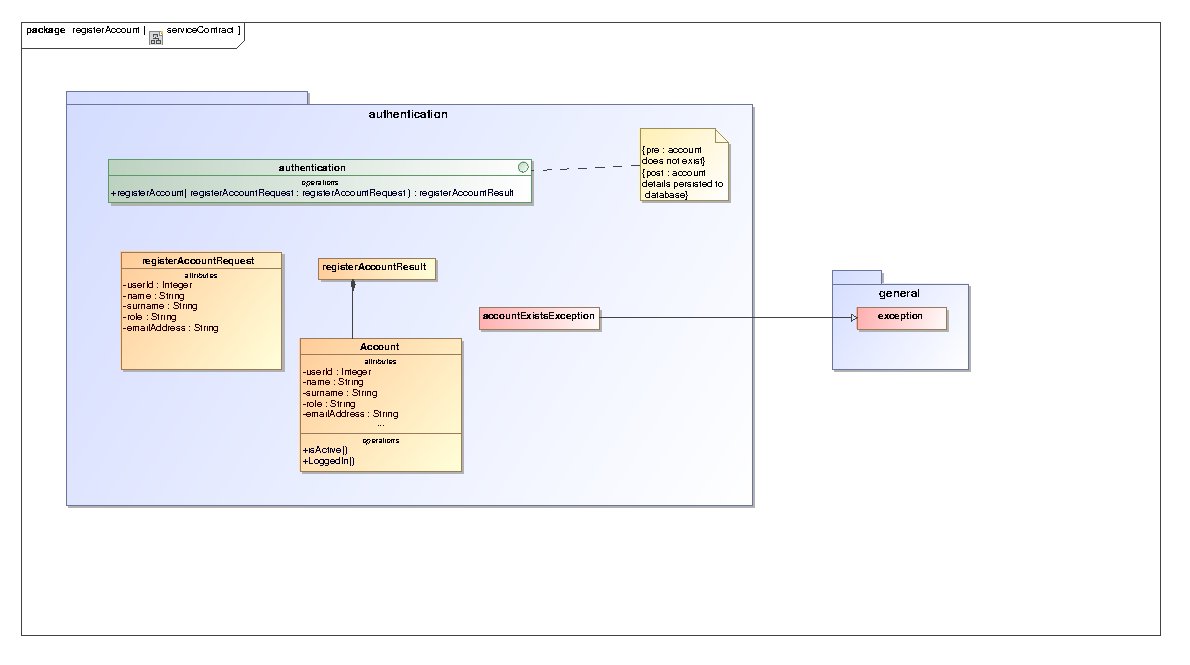
\includegraphics[scale=.9]{epsImages/serviceContract.eps}\\
\item \textbf{Login}
\item \textbf{Logout}
\item \textbf{EditAccount}
\item \textbf{deleteAccount  – priority: important} 
This use case creates  a user account and is persisted through to database.

\par{\textbf{service contract} The service contract for the deleteAccount  service is shown in figure below. The pre-conditions are enforced (raising the appropriate exception should they not be met) and the account of interest is deleted and changes are persisted through to database.}
\\
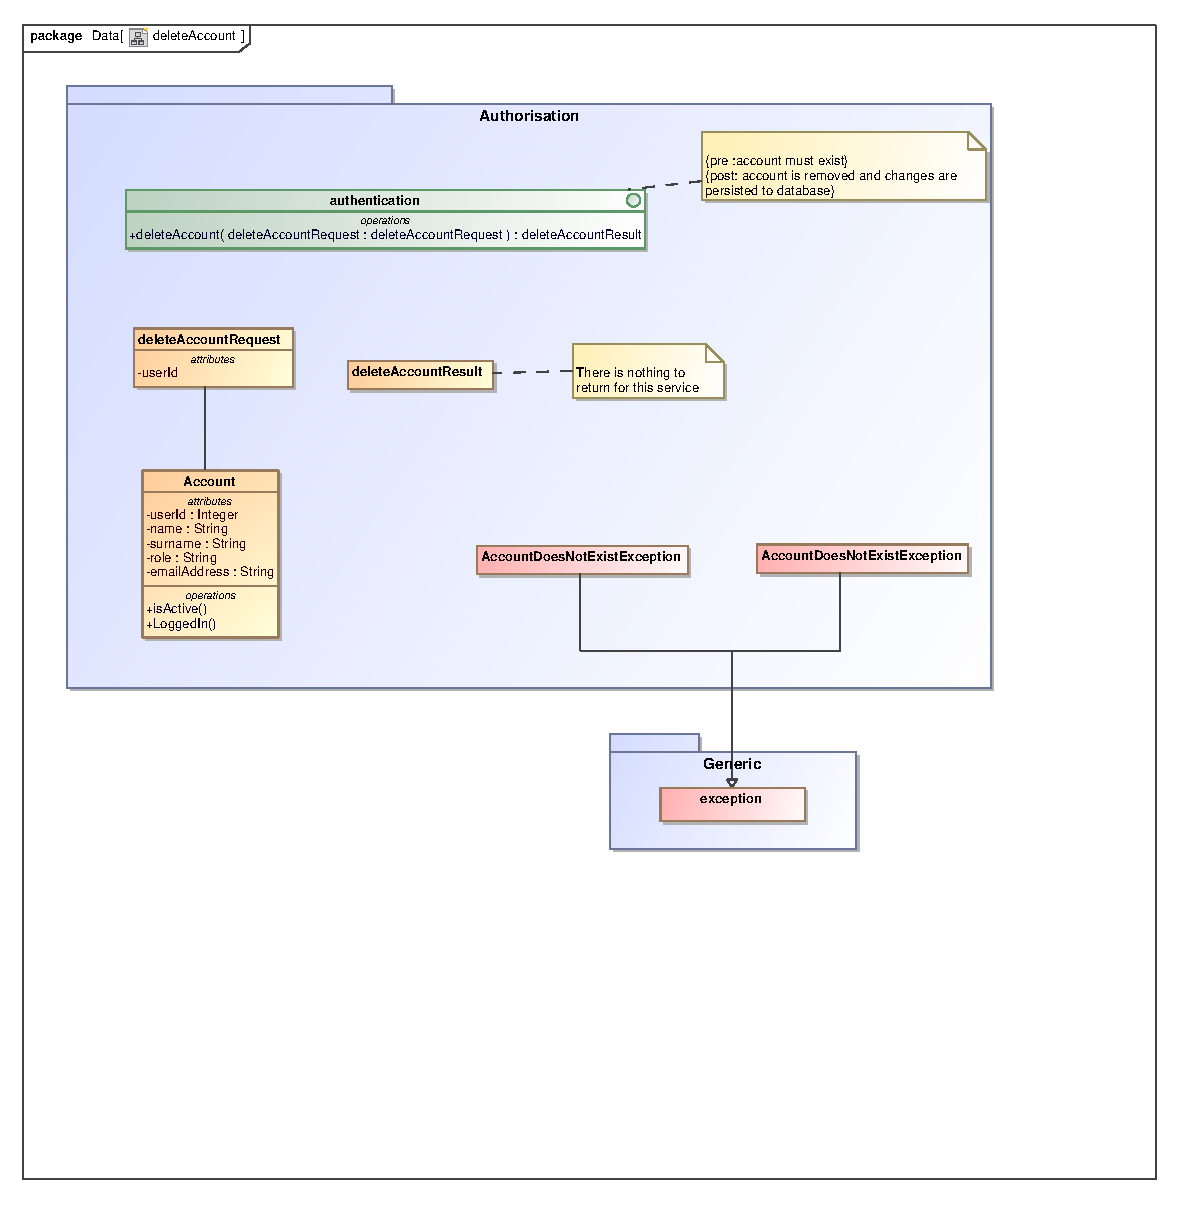
\includegraphics[scale=.9]{epsImages/deleteAccount.eps}\\
\item \bf{SuspendAccount}
\end{enumerate}
\end{document}